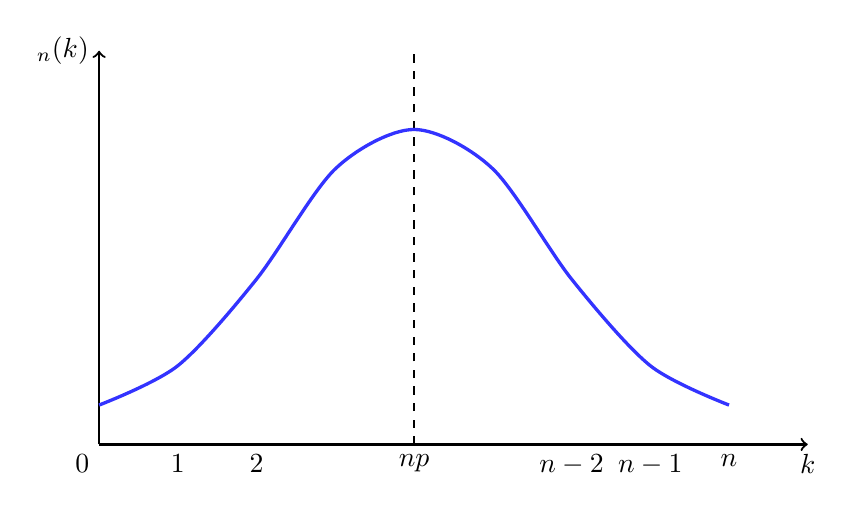
\begin{tikzpicture}
  \draw[->, thick] (0, 0) -- (9, 0)
    node[pos = 1, below] {\(k\)};
  \draw[->, thick] (0, 0) -- (0, 5)
    node[pos = 1, left] {\(\probP_n (k)\)};

  \draw (0, 0) node[below left] {\(0\)};
  \draw (1, 0) node[below] {\(1\)};
  \draw (2, 0) node[below] {\(2\)};
  \draw (3, 0) node[below] {\(\dotsc\)};
  \draw (4, 0) node[below] {\(n p\)};
  \draw (5, 0) node[below] {\(\dotsc\)};
  \draw (6, 0) node[below] {\(n - 2\)};
  \draw (7, 0) node[below] {\(n - 1\)};
  \draw (8, 0) node[below] {\(n\)};

  \draw[thick, dashed] (4, 0) -- (4, 5);
  \draw[very thick, color = blue!80]
    plot[smooth] coordinates {
      (0, 0.5) (1, 1) (2, 2.1) (3, 3.5) (4, 4)
      (5, 3.5) (6, 2.1) (7, 1) (8, 0.5)
    };
\end{tikzpicture}